\section{Reference Sheet}
\subsection{Assumed Knowledge}

\subsubsection{Log Laws}
\begin{gather*}
  \log_b A + \log_b B = \log_b(AB), \\
  \log_b\!\left(\frac{M}{N}\right) = \log_b M - \log_b N, \\
  \log_b(M^k) = k\log_b M, \\
  \log_b(b^k) = k, \\
  b^{\log_b k} = k.
\end{gather*}

\subsubsection{Trig Laws}
\begin{gather*}
  \tan\theta = \frac{\sin\theta}{\cos\theta}, \\
  \cot\theta = \frac{\cos\theta}{\sin\theta}, \\
  \csc\theta = \frac{1}{\sin\theta}, \\
  \sec\theta = \frac{1}{\cos\theta}, \\
  \sin^2\theta + \cos^2\theta = 1, \\
  1 + \cot^2\theta = \csc^2\theta, \\
  \tan^2\theta + 1 = \sec^2\theta, \\
  \sin(A\pm B) = \sin A\cos B \pm \cos A\sin B, \\
  \cos(A\pm B) = \cos A\cos B \mp \sin A\sin B, \\
  \tan(\alpha\pm\beta) = \frac{\tan\alpha \pm \tan\beta}{1 \mp \tan\alpha\tan\beta}.
\end{gather*}

Sine law:
\[
  \frac{\sin A}{a}=\frac{\sin B}{b}=\frac{\sin C}{c}
\]

Cosine law:
\[
  a^2=b^2+c^2-2bc\cos A
\]

\newpage
Unit circle:
\begin{figure}[h!]
  \centering
  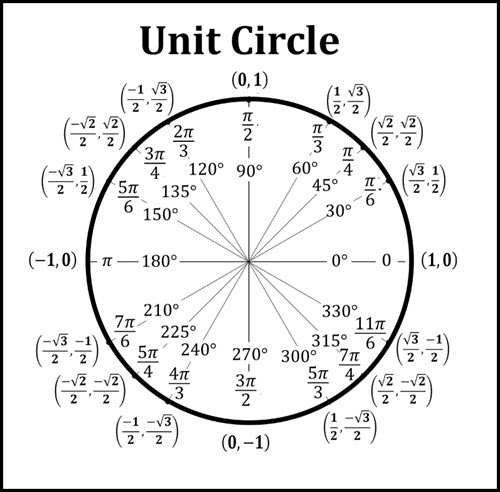
\includegraphics[width=0.8\textwidth]{pictures/unitCircle.jpg}
\end{figure}
